\chapter{量子機械学習におけるコスト関数の勾配の分散の上界}\label{chap:upper-bound}
量子機械学習におけるバレンプラトーの研究は、それ以外の変分量子アルゴリズムにおけるバレンプラトーの研究に比べて少ない\cite{thanasilp2021subtleties,thanasilp2022exponential}。特に、量子機械学習のデータの入力がバレンプラトーにどのように影響するかについては、詳しくわかっていない。そこで、この章では、量子機械学習におけるコスト関数の勾配の分散の上界をデータ入力の観点から調べた結果を示す。
まず、\ref{sec:qml-upper-var}~節では、勾配の分散の上界を、先行研究に基づき新たに導出する。\ref{sec:haar-random-input}~節では、入力状態がグローバルユニタリ $2$--デザインを成す場合の勾配の分散の上界を求める。\ref{sec:qml-var-expressibility}~節では、勾配の分散の上界を入力回路の表現力によって表す。\ref{sec:qml-var-local-2-design}~節では、入力状態がローカルユニタリ $2$--デザインを成すというグローバルユニタリ $2$--デザインよりも弱い仮定の下で、勾配の分散の上界を計算する。最後に、\ref{sec:qml-var-noise}~節では、\ref{sec:qml-var-local-2-design}~節の設定に加えて、Depolarizing ノイズがある場合の勾配の分散の上界を計算する。

本論文のバレンプラトーの解析においては、基本的に図~\ref{fig:qcl-setting}にあるような量子回路学習モデル(\ref{sec:quantum-circuit-learning}~節)を用いる。ただし、定理~\ref{thm:qml-upper-var}については Data reuploading モデル(\ref{sec:data-reuploading}~節)についても成り立つ。
量子カーネル法(\ref{sec:quantum-kernel}~節)に関するバレンプラトーについては、先行研究~\cite{thanasilp2022exponential}において既に解析されているため、本論文では扱わない。
\begin{figure}[H]
    \centering
    \begin{quantikz}
        \lstick{$\ket{0}$}     & \gate[wires=3][3cm]{{\LARGE U(\bs{x}_i)}} & \gate[wires=3][3cm]{{\LARGE V(\bs{\th})}} & \meter{}\\
        \lstick{$\vdots\;\;$}  & \wn &\wn & \wn\rstick{$\vdots$}\\
        \lstick{$\ket{0}$}     &     & \qw & \meter{}
    \end{quantikz}
    \caption{量子回路学習における量子回路の構造}
    \label{fig:qcl-setting}
\end{figure}

$\bs{x}_i$ はデータセット$\{(\bs{x}_i, y_i)\}_{i=1}^N$ の内、$i$ 番目の組の入力に対応するデータであり、$\bs{\th}$ は学習パラメーターである。$U(\bs{x}_i)$ はデータを入力するためのユニタリであり、$V(\bs{\th})$ は学習パラメーターを入力するためのユニタリである。ただし、全てのパラメーター $\bs{\th} = (\th_1,\th_2,
\cdots)$ は独立であり、取りうる区間は $[0, 2\pi]$ であると仮定する。

データ入力後の量子状態の密度演算子を $\rho_i = U(\bs{x}_i)\dyad{\bs{0}}U\dg(\bs{x}_i)$ と表し、これを入力状態と呼ぶ。また、学習パラメーター入力後の量子状態の密度演算子を $\rho_i(\bs{\th}) = V(\bs{\th})U(\bs{x}_i)\dyad{\bs{0}}U\dg(\bs{x}_i)V\dg(\bs{\th})$ とする。

以降の解析においては、$\bbU := \{U(\bs{x})|\,\bs{x}\in \calX \subset \bbR^m,\, m \in \bbN\}$ とする。すなわち、$\bbU$ は入力データ $\bs{x}$ によって生成されるユニタリの集合である。
関数 $g(U(\bs{x}))$ の入力データ $\bs{x}\in \calX$ に関する積分は、次のように $U\in\bbU$ に関する積分として表現する。
\begin{align}
    \int_{\bbU} dU\,g(U) = \int_{\calX} d\bs{x}\,g(U(\bs{x}))
\end{align}


\section{量子機械学習における勾配の分散の一般的な上界}\label{sec:qml-upper-var}
バレンプラトーに関連するほとんどの論文では、コスト関数は式~\eqref{eq:cost-simple} のように、あるオブザーバブルの期待値として与えられる(VQEやQAOAなどの典型的な変分量子アルゴリズムにおけるコスト関数)。一方、教師ありの量子機械学習においては式~\eqref{eq:cost-ml} のように、各訓練データに依存する出力 $\ell_i(\bs{\th})$ それ自体、あるいは更に関数を作用させたものをモデルの予測としてコスト関数が定義される。このようなコスト関数に関するバレンプラトーの先行研究はまだ少ない。
\begin{align}
    \ell_i(\bs{\th}) &= \Tr[\rho_i(\bs{\th})\,O], \label{eq:cost-simple}\\
    \calL(\bs{\th}) &= \frac1N\sum_{i=1}^N f(\ell_i(\bs{\th}),y_i) \label{eq:cost-ml}
\end{align}
ただし、$f$ は $f(x,y) := \abs{x - y}$ や $f(x,y) := (x-y)^2$、$f(x,y) := -y\log{x} - (1-y)\log{(1-x)}$ などの関数であり、
$O$ は任意のオブザーバブルである。
% \memo{この時点で、$\ell_x(\bs{\th}) = \Tr[\rho_x(\bs{\th})\,O]$,$\calL = \E_\calX[f(\ell_i(\bs{\th}),y_i)]$と定義しておけばいいかも\cite{barthe2023gradients}}

$\ell_i(\bs{\th})$ の勾配は、パラメーターシフトルール(\ref{sec:parameter-shift-rule}~節)によって求めることができる。一方、$\calL(\bs{\th})$ の勾配は、$\pd_\nu := \pd/\pd\th_\nu$  として、次のように連鎖律によって求める。
\begin{align}\label{eq:qml-chain-rule}
    \pd_\nu \calL(\bs{\th}) =  \sum_{i=1}^N \pd_{\ell_i(\bs{\th})} f \cdot \pd_\nu \ell_i(\bs{\th}).
\end{align}

この勾配の計算量が量子ビット数に関してどのようにスケールするかを調べることは、量子機械学習の計算量の評価において重要である。よって、バレンプラトーの定義にもあるように、この勾配の分散 $\Var_{V(\bs{\th})}\qty[\pd_\nu \calL(\bs{\th})]$ を調べる。まず、分散の公式を用いて式~\eqref{eq:qml-chain-rule}を次のように変形してみる。
\begin{align}
    \Var_{V(\bs{\th})}\qty[\pd_\nu \calL(\bs{\th})]
    &= \Var_{V(\bs{\th})}\qty[\frac1N\sum_{i=1}^N \pd_\nu f(\ell_i(\bs{\th}),y_i)]\nonumber\\
    &= \frac{1}{N^2} \sum_{i,j=1}^N \Cov_{V(\bs{\th})}[\pd_\nu f(\ell_i(\bs{\th}),y_i), \pd_\nu f(\ell_j(\bs{\th}),y_j)]
\end{align}
すると、$\Var_{V(\bs{\th})}\qty[\pd_\nu \calL(\bs{\th})]$ は $\pd_\nu f(\ell_i(\bs{\th}),y_i)$ の共分散に分解できる。共分散は負の値を取りうるため、$\Var_{V(\bs{\th})}\qty[\pd_\nu \calL(\bs{\th})]$ のスケーリングが $\Var_{V(\bs{\th})}\qty[\pd_\nu \ell_i(\bs{\th})]$ のスケーリングと同じとは限らないことがわかる。

$\Var_{V(\bs{\th})}\qty[\pd_\nu \calL(\bs{\th})]$ の性質に関して、先行研究~\cite{thanasilp2021subtleties}により次の結果が得られている。

\begin{screen}
    \begin{theorem}\label{thm:qml-upper-var-sutlties}
        (論文~\cite{thanasilp2021subtleties}の Theorem 1 の結果)
        量子機械学習におけるコスト関数 $\calL(\bs{\th}) = \sum_{i=1}^N f(\ell_i(\bs{\th};y_i),y_i)$ のパラメーター $\th_\nu \in \bs{\th}$ に関する勾配 $\pd_\nu \calL(\bs{\th}) \equiv \pd \calL(\bs{\th})/\pd \th_\nu$ の分散は次のように上から抑えられる。
        \begin{align}\label{eq:qml-upper-var-sutlties}
            \Var_{V(\bs{\th})}[\pd_\nu\calL(\bs{\th})] \leq \qty(\frac1N \sum_{i=1}^N g_i \sqrt{\Var_{V(\bs{\th})}[\pd_\nu \ell_i(\bs{\th})] + (\E_{V(\bs{\th})}[\pd_\nu \ell_i(\bs{\th})])^2 })^2
        \end{align}
        
        ここで、$\ell_i(\bs{\th}) \equiv \ell_i(\bs{\th};y_i)$ であり、平均と分散はパラメーター $\bs{\th}$ に関して取られている。また、$g_i$ は以下のように定義される。
        \begin{align}
            g_i = \sqrt{2} \max_{\ell_i} \abs{\pdv{f}{\ell_i}}
        \end{align}
        
        ここで、$\max_{\ell_i} \abs{\pd f/\pd \ell_i}$ は $f(\ell_i, y_i)$ の偏微分の絶対値の最大値である。
    \end{theorem}
\end{screen}

この定理は、$\ell_i(\bs{\th})$ の勾配の分散の解析を $\calL(\bs{\th})$ の勾配の分散の解析に適用できることを示した最初の結果であった。例えば、全ての $i$ について $\ell_{i}(\bs{\th})$ がバレンプラトーになるとすると、
\begin{align}
    \E_{V(\bs{\th})}[\pd_\nu\ell_i(\bs{\th})] = 0, \quad
    \Var_{V(\bs{\th})}[\pd_\nu\ell_i(\bs{\th})] \in \order{2^{-\alpha\,n}},\quad 0<\alpha \quad \text{for all $i$}
\end{align}
が成り立つ。よって、全ての $i$ について $g_{i} \in \order{\poly(n)}$ であるならば、上界~\eqref{eq:qml-upper-var-sutlties}は $\order{2^{-\alpha\,n}}$ となる。したがって、$\calL(\bs{\th})$ もバレンプラトーとなる。

本研究では、上界について次の定理\ref{thm:qml-upper-var}を導いた。
上界\eqref{eq:qml-upper-var-1}は上界\eqref{eq:qml-upper-var-sutlties}よりも緩いが、具体的な回路に対して上界を解析的に計算することができる。
\begin{screen}
    \begin{theorem}\label{thm:qml-upper-var}
        Theorem \ref{thm:qml-upper-var-sutlties}と同じ仮定の下、次の不等式が成り立つ。
        \begin{align}\label{eq:qml-upper-var-1}
            \Var_{V(\bs{\th})}[\pd_\nu \calL(\bs{\th})]
            &\leq
            2\max_{i,\bs{\th}} [(\pd_{\ell_i(\bs{\th})}f)^2]
            \times
            % \frac1N\sum_i \Var[\pd_\nu \ell_i(\bs{\th})]
            \int_{U\in\bbU} dU \Var_{V(\bs{\th})}[\pd_\nu \ell(\bs{\th})]
        \end{align}
    \end{theorem}
\end{screen}

この定理の証明においては、次の補題を用いる。証明は論文\cite{thanasilp2022exponential}の Lemma 1, 5 を参照されたい。
\begin{screen}
    \begin{lemma}\label{lem:variance-inequality}
        分散についての以下の不等式が成り立つ。
        \begin{align}
            \Var\Big[\sum_i X_i\Big] &\leq N\sum_i\Var[X_i],\label{eq:sum-variance}\\
            \Var[XY] &\leq 2\Var[X]\abs{Y^2}_{\max} + 2(\E[X])^2\Var[Y]\,.\label{eq:prod-variance}
        \end{align}
    \end{lemma}
\end{screen}

\begin{proof}\label{proof:qml-upper-var}
    まず、$\E_{V(\bs{\th})}\qty[\pd_\nu \ell_i(\bs{\th})] = 0$ を示す。ここでは、定理\ref{thm:bp}と同じように、$\ell_i(\bs{\th}) := C(\bs{\th}) = \Tr[\rho_i(\bs{\th})O]$, $V(\bs{\th}) = V_+V_-$, $V_+ := \prod_{l=k+1}^L U_l(\th_l)W_l$, $V_- := \prod_{l=1}^{k} U_l(\th_l)W_l$ とする。また、証明~\ref{proof:bp}で得られるように、次の等式が成り立つ。
    \begin{align}
        \pd_\nu \ell_i(\bs{\th})
        &=\frac{i}{2}\Tr[V_-\rho V_-\dg\, [P_k, V_+\dg OV_+]]
    \end{align}
    
    簡単のため、 $c = \cos(\th_\nu/2),\, s = \sin(\th_\nu/2)$ とする。このとき、$\pd_\nu \ell_i(\bs{\th})$ は次のように展開できる。
    \begin{align}
        \pd_\nu \ell_i(\bs{\th})
        &= \frac{i}{2}\Tr[V_-\rho V_-\dg\, [P_k, V_+\dg OV_+]]\\
        &= \frac{i}{2}\Tr[\qty(c\,\bbid - i\,sP_k)W_k\qty(\prod_{l=1}^{k-1}U_lW_l)\rho \qty(\prod_{l=1}^{k-1}U_lW_l)\dg W_k\dg\qty(c\,\bbid - i\,sP_k)\dg\, [P_k, V_+\dg OV_+]]\\
        &= \frac{i}{2}\qty{(c^2-s^2)\Tr[[\rho^\prime, P_k]V_+\dg OV_+] + i\,cs\Tr[[\rho^\prime, P_k]]}
    \end{align}
    ただし、$\rho^\prime = W_k\qty(\prod_{l=1}^{k-1}U_lW_l)\rho \qty(\prod_{l=1}^{k-1}U_lW_l)\dg W_k\dg$ とした。
    $\th_\nu \in [0,2\pi]$ による平均は、
    \begin{align}
        \frac{1}{2\pi}\int_0^{2\pi} d\th_\nu\, (c^2-s^2) = 0, \quad
        \frac{1}{2\pi}\int_0^{2\pi} d\th_\nu\, cs = 0
    \end{align}
    である。よって、$\E_{V(\bs{\th})}\qty[\pd_\nu \ell_i(\bs{\th})] = 0$ である。
    
    次に $\Var_{V(\bs{\th})}[\pd_\nu \calL(\bs{\th})]$ の上界を導く。
    \begin{align}
        \Var_{V(\bs{\th})}\qty[\pd_\nu \calL(\bs{\th})]
        &= \Var_{V(\bs{\th})}\qty[\frac1N\sum_{i=1}^N \pd_\nu f(\ell_i(\bs{\th}),y_i)]\\
        &\overset{(1)}{\leq} \frac1N\sum_{i=1}^N \Var_{V(\bs{\th})}[\pd_\nu f(\ell_i(\bs{\th}),y_i)]\\
        &= \frac1N\sum_{i=1}^N \Var_{V(\bs{\th})}[\pd_{\ell_i(\bs{\th})}f \cdot \pd_\nu \ell_i(\bs{\th})]\\
        &\overset{(2)}{\leq} \frac1N\sum_{i=1}^N 2\max_{\bs{\th}}[(\pd_{\ell_i(\bs{\th})}f)^2] \cdot \Var_{V(\bs{\th})}[\pd_\nu \ell_i(\bs{\th})]\\
        &\leq 2\max_{i,\,\bs{\th}}[(\pd_{\ell_i(\bs{\th})}f)^2] \times \frac1N\sum_{i=1}^N \Var_{V(\bs{\th})}[\pd_\nu \ell_i(\bs{\th})]\\
        &=: 2\max_{i,\bs{\th}} [(\pd_{\ell_i(\bs{\th})}f)^2]
        \times \int_{U\in\bbU} dU \Var_{V(\bs{\th})}[\pd_\nu \ell(\bs{\th})]
    \end{align}
    
    ただし、不等式(1)では、不等式\eqref{eq:sum-variance}を用いた。不等式(2)では、不等式\eqref{eq:prod-variance}と $\E_{V(\bs{\th})}\qty[\pd_\nu \ell_i(\bs{\th})] = 0$ を用いた。
\end{proof}


この結果から、コスト関数の勾配の分散の上界を求めるためには、$\int_{U\in\bbU} dU \Var_{V(\bs{\th})}[\pd_\nu \ell(\bs{\th})]$ を計算する必要があるとわかる。具体的なスケーリングを求めるため、以降の解析においては、図~\ref{fig:circuit-setting}の構造を仮定する。すなわち、初めは入力回路には条件を課さず、学習回路のみ $\xi$ 個の $s$ 量子ビットユニタリのテンソル積からなる回路であるとする。
\begin{figure}[H]
    \centering
    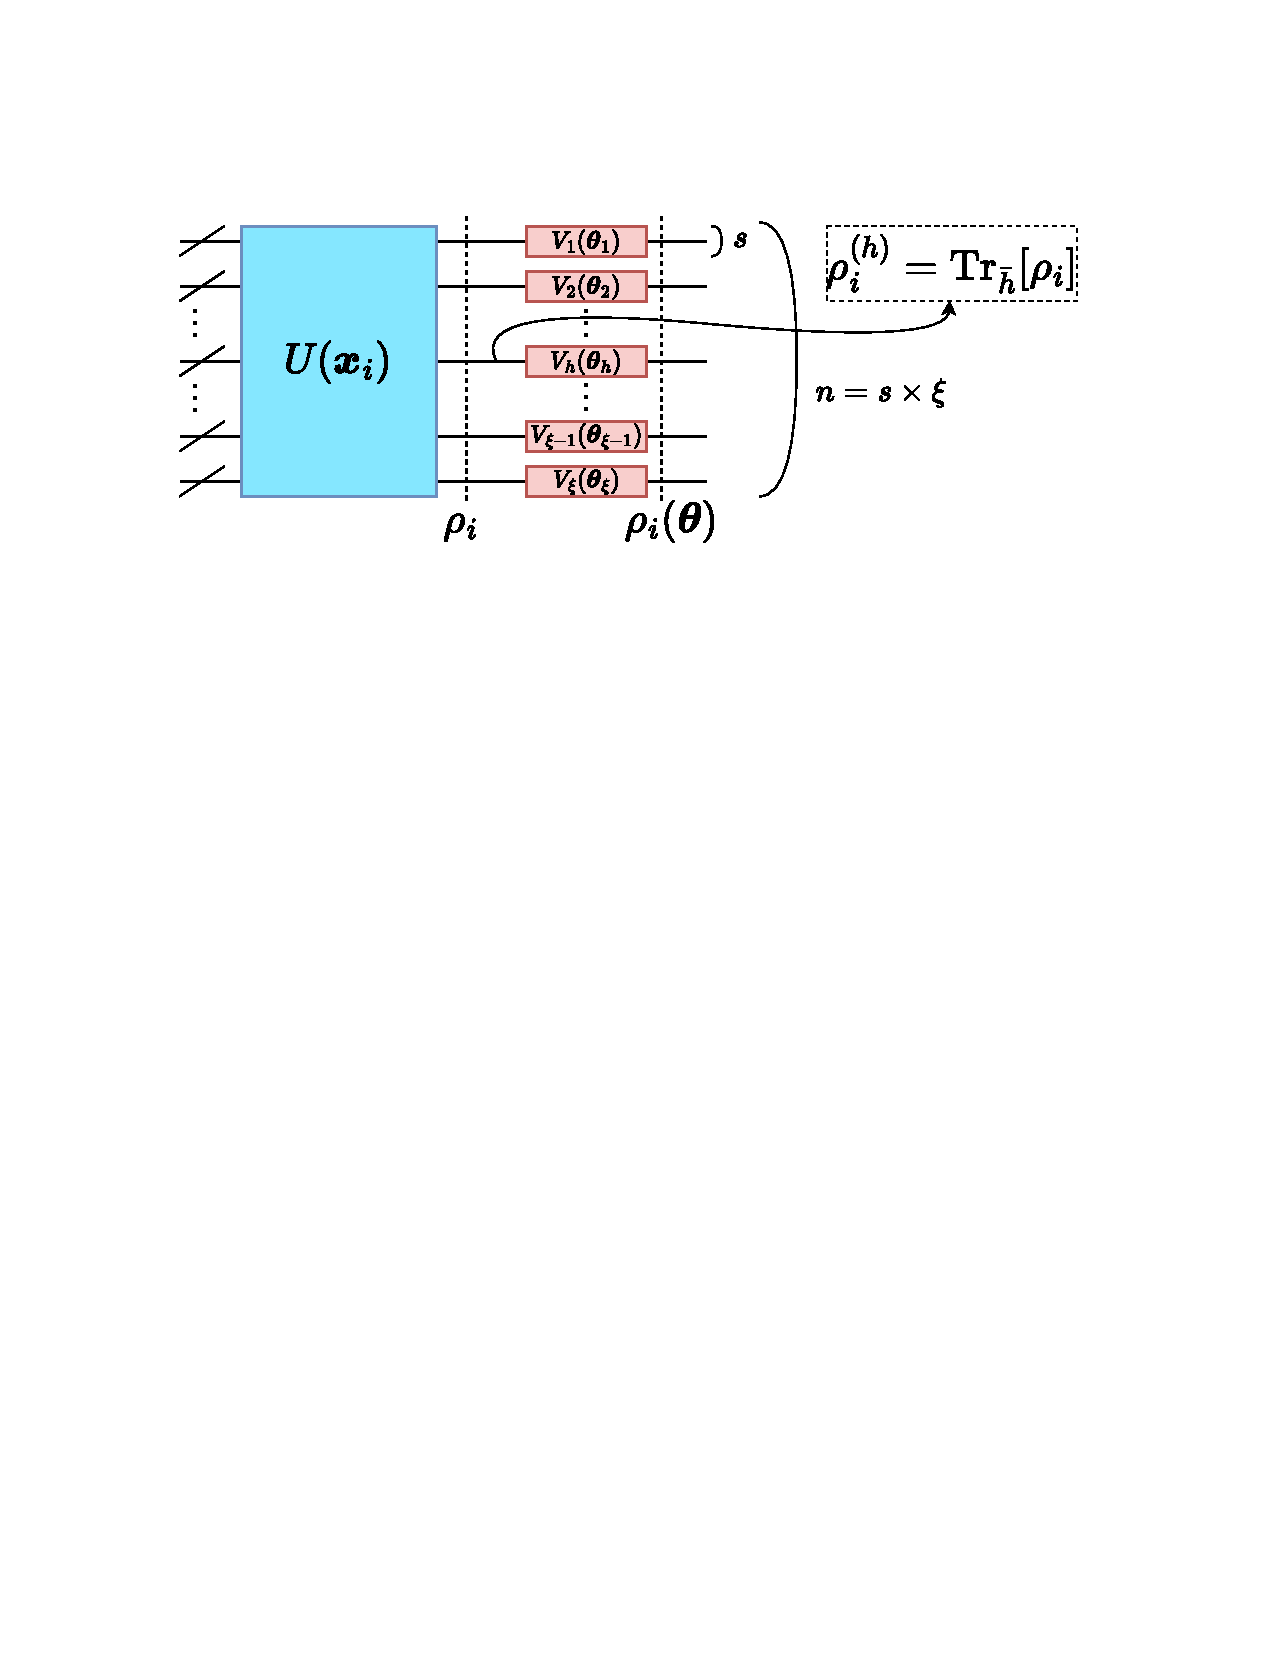
\includegraphics[width=16cm]{setting.pdf}
    \caption{解析する量子回路の構造:学習回路は $s$ 量子ビットユニタリのテンソル積からなる}
    \label{fig:circuit-setting}
\end{figure}

この学習回路の各 $s$ 量子ビットユニタリがそれぞれユニタリ $2$--デザインを成す、すなわち、ローカルユニタリ $2$--デザインを成すと仮定する。
このとき、次の命題が成り立つことが先行研究~\cite{cerezo2021cost}により示されている。
\begin{screen}
    \begin{proposition}\label{prop:qml-var-local-2-design}
        (論文~\cite{cerezo2021cost}の Supplementary Note 5, B の結果) 
        $V(\bs{\th})$ が、$s$ 量子ビットユニタリのテンソル積からなり、それぞれがローカルユニタリ $2$--デザインを成すと仮定する。コスト関数 $\ell_i(\bs{\th}) = \Tr[\rho_i(\bs{\th})O_\rmL],\,O_\rmL = \frac{1}{n} \sum_{j=1}^{n}\dyad{0}_{j} \otimes \bbid_{\bar{j}}$ について、$h$ 番目のゲートブロック中のパラメーター $\th_\nu$ 関する偏微分を考える。このとき、次の等式が成り立つ。
        \begin{align}
            \Var_{V(\bs{\th})}[\pd_\nu \ell_i(\bs{\th})] = r_{n,s}D_{\HS}(\rho_i^{(h)} , \bbid/2^s )\label{eq:ell-var}
        \end{align}
        ここで、$r_{n,s} := \frac{s\cdot 2^{3(s-1)}}{n^2(2^{2s}-1)^2} \in \Omega(1/\poly(n))$ であり、$D_{\HS}(A, B) = \Tr[(A - B)^2]$ は Hilbert--Schmidt 距離である。また、$\bbid/2^s$ は $s$ 量子ビット上の最大混合状態であり、$\rho_i^{(h)} = \Tr_{\bar h}[U(\bs{x}_i)\dyad{\bs{0}}U\dg(\bs{x}_i)]$ は $h$ 番目のユニタリが作用する $s$ 量子ビット上の入力状態の縮約密度演算子である。
    \end{proposition}
\end{screen}

この命題において、学習回路とオブザーバブルの情報は $r_{n,s}$ に含まれるが、$s$ は $n$ によらず、オブザーバブルは局所的なものであるため、これらはバレンプラトーの原因とならない。
一方で、この命題は、入力状態の縮約密度演算子 $\rho_i^{(h)}$ が最大混合状態に近いほど、$\Var_{V(\bs{\th})}[\pd_\nu \ell_i(\bs{\th})]$ が小さくなることを意味する。つまり、式~\eqref{eq:ell-var}は、データセットと入力回路の構造の情報を含む $\rho_i$ がバレンプラトーを引き起こす可能性があることを意味する。

式~\eqref{eq:ell-var}を式~\eqref{eq:qml-upper-var-1}に代入すると、次の上界を得る。
\begin{align}\label{eq:qml-upper-var-2}
    \Var_{V(\bs{\th})}[\pd_\nu \calL(\bs{\th})]
    &\leq
    2\max_{i,\bs{\th}} [(\pd_{\ell_i(\bs{\th})}f)^2]
    \times r_{n,s} \times
    \int_{U\in\bbU} dU D_{\HS} (\rho^{(h)} , \bbid/2^s ).
\end{align}

よって、$\int_{U\in\bbU} dU D_{\HS} (\rho^{(h)} , \bbid/2^s)$ が上界のスケーリングを決めることがわかる。

\begin{comment}
    \section{Connect two papers results}
    \cite{cerezo2021cost,thanasilp2021subtleties}When QNN is giben by a single layer of the alternating layered ansatz made of a tensor product of s-qubit unitaries and a local cost function is
    $$
        \ell_i(\bs{\th}) = 1 - \frac{1}{n}\sum_{j=1}^n \Tr[(\dyad{0}_j \ot \bbid_{\bar{j}} ) \rho_i(\bs{\th})] ,
    $$
    the $\Var_{V(\bs{\th})}[\pd_\nu\, \ell_i(\bs{\th})]$ is given by

    \begin{align}
        \Var_{V(\bs{\th})}[\pd_\nu\, \ell_i(\bs{\th})] = r_{n,s}\,D_{\HS}(\rho_i^{(h)},\, \bbid/2^s),\quad r_{n,s} = \frac{s\cdot 2^{3(s-1)}}{n^2(2^{2s}-1)^2} \in \Omega\qty(\frac{1}{\poly(n)}).
    \end{align}

    Using the inequality in \textbf{Theorem 2}, $\Var_{V(\bs{\th})}[\pd_\nu\, \ell_i(\bs{\th})]$ is bounded as follows.
    \begin{align}
        \frac{r_{n,s}}{d}\,D_2(\rho_i^{(h)},\, \bbid/2^s) \leq \Var_{V(\bs{\th})}[\pd_\nu\, \ell_i(\bs{\th})] \leq \frac{r_{n,s}}{e}\,D_2(\rho_i^{(h)},\, \bbid/2^s).
    \end{align}

    In a kind of circuits, $D_2(\rho,\, \bbid/2^s)$ is shown to be exponentially small with respect to the number of embedding layers~\cite{thanasilp2022exponential}.
    We have to note that the some assumptions are different in these two papers~\cite{thanasilp2022exponential,cerezo2021cost}. However, If we were able to show that $\bbV[\pd_\nu\, \ell_i(\bs{\th})]$ is given by the form of $r_{n,s}\,D_{\HS}(\rho_i,\, \bbid/2^s)$ and $D_2(\rho_i,\, \bbid/2^s) \in \Omega\qty(e^{-\alpha n})\, (\alpha>0)$ for the same conditions, it shows the effect of encoding on barren plateaus.
\end{comment}



\section{グローバルユニタリ $2$--デザインの入力状態とバレンプラトー}\label{sec:haar-random-input}
バレンプラトーの解析においては、しばしば、学習回路がグローバルユニタリ $2$--デザインを成すと仮定する。そこで、$\int_{U\in\bbU} dU D_{\HS} (\rho^{(h)} , \bbid/2^s)$ を計算する最初の簡単なモデルとして、入力状態の集合がグローバルユニタリ $2$--デザインを成すと仮定する。
$D_{\HS} (\rho , \bbid/2^s) = \Tr[\rho^2] - 1/2^s$ であることから、
\begin{align}
    D_{\HS}(\rho^{(h)},\bbid/2^s) = \Tr[(\Tr_{\bar{h}}[U\dyad{\bs{0}} U\dg])^2] - 1/2^s
\end{align}
であり、最初の項は $U,\,U\dg$ の成分に関してそれぞれ2次の多項式である。よって、ユニタリ $2$--デザインの定義から次のように $\bbU = \calU(d),\, dU = d\mu_{\Haar}(U)$ として積分してよい。
\begin{align}
    \int_{U\in\calU(d)} d\mu_{\Haar}(U) D_{\HS}(\rho^{(h)},\bbid/2^s)
    = \int_{U\in\calU(d)} d\mu_{\Haar}(U) \Tr[(\Tr_{\bar{h}}[U\dyad{\bs{0}} U\dg])^2] - 1/2^s 
\end{align}
となる。右辺の第一項の積分計算は、次の定理により与えられる。

\begin{screen}
    \begin{theorem}\label{thm:dhs-haar-int}
        $\calH$ を $\calH = \calH_h \ot \calH_{\overline{h}}$ のように二つの系からなる $n$ 量子ビットの Hilbert 空間とする。ここで、$\calH_h$ は $s$ 量子ビットからなる Hilbert 空間であり、$\calH_{\overline{h}}$ は残りの $n-s$ 量子ビットからなる Hilbert 空間である。このとき、次の式が成り立つ。
        \begin{align}
            \int_{U\in\calU(d)}\Tr_h[(\Tr_{\bar{h}}[U\dyad{\bs{0}}U\dg])^2] dU
            =
            \frac{2^{n-s} + 2^{s}}{2^n+1}.
        \end{align}
    \end{theorem}
\end{screen}

\begin{proof}
    $ a_{ij} = U_{i1}U_{j1}^*,\,\,t = 2^{n-s}$ とすると、
    \begin{align}
        &\Tr_{\bar{h}}[U\dyad{\bs{0}}U\dg]=\nonumber\\
        &\begin{bmatrix}
            a_{1,1}+a_{2,2}+\cdots+a_{t,t} & a_{1,t+1}+a_{2,t+2}+\cdots+a_{t,2t}& \cdots & a_{1,2^n-t+1}+a_{2,2^n-t+2}+\cdots+a_{t,2^n}\\
            a_{t+1,1}+a_{t+2,2}+\cdots+a_{2t,t} & a_{t+1,t+1}+a_{t+2,t+2}+\cdots+a_{2t,2t} & \cdots & a_{t+1,2^n-t+1}+a_{t+2,2^n-t+2}+\cdots+a_{2t,2^n}\\
            \cdots & \cdots & \cdots & \cdots\\
            a_{2^n-t+1,1}+\cdots+a_{2^n,t} & a_{2^n-t+1,t+1}+\cdots+a_{2^n,2t} & \cdots & a_{2^n-t+1,2^n-t+1}+\cdots+a_{2^n,2^n}.
        \end{bmatrix}
    \end{align}
    よって、上の行列の二乗 $(\Tr_{\bar{h}}[U\dyad{\bs{0}}U\dg])^2$ の(1,1)成分は以下のようになる。
    \begin{align}
        (a_{1,1}+a_{2,2}+\cdots+a_{t,t})^2 + (a_{1,t+1}+a_{2,t+2}+\cdots+a_{t,2t})(a_{t+1,1}+a_{t+2,2}+\cdots+a_{2t,t})\nonumber\\
        \cdots + (a_{1,2^n-t+1}+\cdots+a_{t,2^n})(a_{2^n-t+1,1}+\cdots+a_{2^n,t})
    \end{align}
    
    ユニタリ $2$--デザインの定義から、ハール分布の積分公式~\eqref{eq:haar-int-2}を用いることができ、
    \begin{align}
        \int_{U\in\calU(d)}d\mu_{\Haar}(U)\,a_{ij}a_{i^\prime j^\prime} = \frac{1}{d(d+1)}(\delta_{ij}\delta_{i^\prime j^\prime} + \delta_{ij^\prime}\delta_{i^\prime j})
    \end{align}
    が成り立つ。よって、$a_{p,p}a_{p,p},\,a_{p,p}a_{q,q},\,a_{p,q}a_{q,p}\,(p \neq q)$ のみが生き残る。他の対角成分も同様であるから、求める式は以下のようになる。
    
    \begin{align}
        &\int_{U\in\calU(d)}\Tr[(\Tr_{\bar{h}}[U\dyad{\bs{0}}U\dg])^2] d\mu_{\Haar}(U)\nonumber\\
        &=\int_{U\in\calU(d)}d\mu_{\Haar}(U)
        \qty(
            \qty[\sum_{i=1}^t a_{ii}^2]
            + \qty[2\sum_{i<j}^t a_{ii}a_{jj}]
            + \underbrace{\qty[\sum_{i=1}^t a_{t+i,i}a_{i,t+i}] + \cdots + \qty[\sum_{i=1}^t a_{2^n-t+i,i}a_{i,2^n-t+i}]}_{2^s-1 \text{ 個}}
        ) \times 2^s\\
        &=\int_{U\in\calU(d)}d\mu_{\Haar}(U) \qty(\qty[\sum_{i=1}^t a_{ii}^2] + \qty[2\sum_{i<j}^t a_{ii}a_{jj}] + \qty[\sum_{i=1}^t a_{t+i,i}a_{i,t+i}] \times (2^s - 1)) \times 2^s\\
        &=\qty(t\times \frac{2}{d(d+1)} + 2\times \combi{t}{2}\times\frac{1}{d(d+1)} + t\times \frac{1}{d(d+1)} \times (2^s - 1)) \times 2^s\\
        &=\frac{2^{n-s} + 2^s}{2^n + 1}
    \end{align}
    
    % \footnote{他の証明方法については、公式~\eqref{fig:haar-int-4}、論文~\cite{low2009large} の Lemma 4.1、論文~\cite{zhang2014matrix} の Remark 3.12、論文~\cite{zhang2022fundamental} の Corollary S3 を参照。}
\end{proof}


この定理より、
\begin{align}
    \int_{U\in\calU(d)} d\mu_{\Haar}(U) D_{\HS}(\rho^{(h)},\bbid/2^s)
    &= \int_{U\in\calU(d)} d\mu_{\Haar}(U) \Tr[(\Tr_{\bar{h}}[U\dyad{\bs{0}} U\dg])^2] - 1/2^s \nonumber\\
    &= \frac{2^{n-s} + 2^s}{2^n + 1} - 1/2^s \nonumber\\
    &= \frac{2^s - 2^{-s}}{2^n + 1} \,\in [0,1 - 1/2^s]\\
    &=: \calD_{\Haar}
\end{align}

したがって、入力状態の集合がグローバルユニタリ $2$--デザインを成す場合の上界は次で与えられる。
\begin{align}\label{eq:qml-upper-var-haar}
    \Var_{V(\bs{\th})}[\pd_\nu \calL(\bs{\th})]
    &\leq
    2\max_{i,\bs{\th}} [(\pd_{\ell_i(\bs{\th})}f)^2]
    \times r_{n,s}
    \times \frac{2^s - 2^{-s}}{2^n + 1} \,\in \order{\frac{1}{2^n}}
\end{align}
以上より、量子回路の構造は図~\ref{fig:circuit-setting}で与えられ、学習回路やオブザーバブルがパレンプラトーを引き起こさないとしても、入力状態の集合がグローバルユニタリ $2$--デザインを成す場合は、コスト関数はバレンプラトーとなることが分かった。



\section{入力回路の表現力による上界}\label{sec:qml-var-expressibility}
この節では、上界\eqref{eq:qml-upper-var-2} のうち $\int_{U\in\bbU} dU D_{\HS} (\rho^{(h)} , \bbid/2^s )$ の項が、前節で得た結果 
$$
    \calD_{\Haar} = \frac{2^s - 2^{-s}}{2^n + 1}
$$
と入力回路の表現力によって、次のように上から抑えられることを示す。
$$
    \int_{U\in\bbU} dU D_{\HS} ( \rho^{(h)} ,\, \bbid/2^s ) \leq \calD_{\Haar} + \epsilon_{\bbU}^{(2,1)}(\dyad{0})
$$
この不等式により、入力回路の表現能力が高いほど、上界がきつくなることが定性的に理解される。

まず、その証明に必要な2つの補題を示す。
\begin{screen}
    \begin{lemma}\label{lemma:swap1}
        密度演算子 $\rho_A \in \calS(\calH_A)  ,\,\rho_B \in \calS(\calH_B) \; (\dim{\calH_A} = \dim{\calH_B})$ に対して、次の等式が成り立つ。
        \begin{align}\label{eq:swap1}
            \Tr_A[\SWAP\,(\rho_A \ot \rho_B)] = \rho_A\,\rho_B
        \end{align}
        ただし、$\SWAP := \sum_{i,j=1}^d \kten{i}{j}\bten{j}{i}, \eg \SWAP\,\kten{x_i}{y_j} = \kten{y_j}{x_i}$ である。
    \end{lemma}
\end{screen}

\begin{proof}
    $\rho_A$ と $\rho_B$ は、それぞれ $\rho_A = \sum_{i=1}^d \lambda_i \dyad{x_i}$ と $\rho_B = \sum_{i=1}^d \mu_i \dyad{y_i}$ のように固有分解されると仮定する。これを $\Tr_A[\SWAP\,(\rho_A \ot \rho_B)]$ に代入すると、
    \begin{align*}
        \Tr_A[\SWAP\,(\rho_A \ot \rho_B)]
        &= \Tr_A\qty[\SWAP\,\qty(\sum_{i,j=1}^d \lambda_i \mu_j (\kten{x_i}{y_j})(\bten{x_i}{y_j}))]\\
        &= \Tr_A\qty[\sum_{i,j=1}^d \lambda_i \mu_j (\kten{y_j}{x_i})(\bten{x_i}{y_j})]\\
        &= \sum_{i,j=1}^d \lambda_i \mu_j \Tr_A[\dyad{y_j}{x_i}]\,\dyad{x_i}{y_j}\\
        &= \sum_{i,j=1}^d \lambda_i \mu_j \braket{x_i}{y_j}\ketbra{x_i}{y_j}\\
        &= \rho_A\,\rho_B
    \end{align*}
\end{proof}


\begin{screen}
    \begin{lemma}\label{lemma:swap2}
        密度演算子 $\rho_{C1} \in \calS(\calH_{C1} = \calH_{A1} \ot \calH_{B1}),\;\rho_{C2} \in \calS(\calH_{C2} = \calH_{A2} \ot \calH_{B2}) \;(\dim\calH_{A1} = \dim\calH_{A2},\,\,\dim\calH_{B1} = \dim\calH_{B2}$) に対して、次の等式が成り立つ。
        \begin{align}
            \Tr[\Tr_{B1}\rho_{C1} \times \Tr_{B2}\rho_{C2}]
            = \Tr[(\SWAP_{A1,A2} \ot \bbid_{B1,B2})\,(\rho_{C1} \ot \rho_{C2})]
        \end{align}
    \end{lemma}
\end{screen}

\begin{proof}
    \begin{align*}
        \Tr_{B1}\rho_{C1} \times \Tr_{B2}\rho_{C2}
        &\overset{(1)}{=} \Tr_{A1}[\SWAP_{A1,A2}\,(\Tr_{B1}\rho_{C1} \ot \Tr_{B2}\rho_{C2})]\\
        &= \Tr_{A1}[\SWAP_{A1,A2}\,\Tr_{B1,B2}[\rho_{C1} \ot \rho_{C2}]]\\
        &\overset{(2)}{=} \Tr_{A1,B1,B2}[(\SWAP_{A1,A2} \ot \bbid_{B1,B2})\,(\rho_{C1} \ot \rho_{C2})]\\
        &= \Tr_{C1,B2}[(\SWAP_{A1,A2} \ot \bbid_{B1,B2})\,(\rho_{C1} \ot \rho_{C2})].
    \end{align*}
    等式(1)では、補題\ref{lemma:swap1}を用いた。
    等式(2)では、任意の $V,W \in \calL(\calH_{AB})$ に対して、$\Tr_A[V\Tr_B[W]] = \Tr_{AB}[(V \ot \bbid_B) W]$ が成り立つことを用いた。最後に、残りの系 $A_2$ についてトレースを取ればよい。
\end{proof}



これら2つの補題を用いて、次の定理を示す。
\begin{screen}
    \begin{theorem}\label{thm:qml-var-expressibility}
        図~\ref{fig:circuit-setting}の量子回路を用い、入力状態には何も仮定せす、学習回路の $s$ 量子ビットユニタリはそれぞれローカルユニタリ $2$--デザインを成すと仮定する。このとき、
        $\int_{U\in\bbU}dU D_{\HS} (\rho^{(h)} ,\, \bbid/2^s )$ は
        $\calD_{\Haar} := \frac{2^s - 2^{-s}}{2^n+1}$
        と入力回路の表現力 $\epsilon_{\bbU}^{(t,p)}(\cdot)$ によって次のように上から抑えられる。
        \begin{align}
            \int_{U\in\bbU}dU D_{\HS} (\rho^{(h)} ,\, \bbid/2^s )
            &\leq \calD_{\Haar} + \epsilon_{\bbU}^{(2,1)}(\dyad{\bs{0}})\\
            &\leq \calD_{\Haar} + 2^n\epsilon_{\bbU}^{(2,2)}(\dyad{\bs{0}}).
        \end{align}
    \end{theorem}
\end{screen}


\begin{proof}
    $\calA_{\bbU}^{(t)}(X)$ の定義\ref{def:expressibility}において、$t=2,\,X = \dyad{\bs{0}}$ とすると、
    \begin{align}
        \int_{U\in\bbU} dU\,(U\dyad{\bs{0}}U\dg)\otn{2} &= \int_{U\in\calU(d)} d\mu_{\Haar}(U)\,(U\dyad{\bs{0}}U\dg)\otn{2} - \calA_{\bbU}^{(2)}(\dyad{\bs{0}})
    \end{align}
    であるから、$\rho = U\dyad{\bs{0}}U\dg$ として、両辺に $\SWAP_{h_1, h_2}$ を作用させてトレースを取ると
    \begin{align}
        \int_{U\in\bbU} dU\,\Tr[(\rho \ot \rho)\,\SWAP_{h_1, h_2}]
        &= \int_{U\in\calU(d)} d\mu_{\Haar}(U)\,\Tr[(\rho \ot \rho)\,\SWAP_{h_1, h_2}] \nonumber\\
        &\quad - \Tr[\calA_{\bbU}^{(2)}(\dyad{\bs{0}})\,\SWAP_{h_1, h_2}]
    \end{align}
    
    補題\ref{lemma:swap2} より等式 $\Tr[(\rho \ot \rho)\,\SWAP_{h_1, h_2}] = \Tr[(\rho^{({h})})^2]$ が成り立つから 
    \begin{align}
        \int_{U\in\bbU} dU\,\Tr[(\rho^{({h})})^2]
        &= \int_{U\in\calU(d)} d\mu_{\Haar}(U)\,\Tr[(\rho^{({h})})^2] - \Tr[\calA_{\bbU}^{(2)}(\dyad{\bs{0}})\,\SWAP_{h_1, h_2}]
    \end{align}
    
    したがって、
    \begin{align}
        \abs{
            \int_{U\in\bbU} dU \Tr\qty[(\rho^{({h})})^2] - \frac{1}{2^s}
        }
        &= \abs{
            \int_{U\in\calU(d)}\mathrm{d}\mu_{\Haar}(U)
            \Tr\qty[(\rho^{(h)})^2] -\frac{1}{2^s}
            - \Tr\qty[\calA^{(2)}_{\bbU}(\rho)\,\SWAP_{h_1,h_2}]
        }\\
        &\overset{(1)}{\leq} \abs{
            \int_{U\in\calU(d)}\mathrm{d}\mu_{\Haar}(U)
            \Tr\qty[(\rho^{(h)})^2] - \frac{1}{2^s}
        }
        + \abs{
            \Tr\qty[\calA_{\bbU}^{(2)}(\rho)\,\SWAP_{h_1,h_2}]
        }\\
        &\overset{(2)}{\leq} \calD_{\Haar} + \|\calA_{\bbU}^{(2)}(\rho)\|_1 \norm{\SWAP_{h_1,h_2}}_{\infty}\\
        &\overset{(3)}{=} \calD_{\Haar} + \|\calA_{\bbU}^{(2)}(\rho)\|_1\\
        &\overset{(4)}{\leq} \calD_{\Haar} + 2^n\|\calA_{\bbU}^{(2)}(\rho)\|_2
    \end{align}
    不等式(1)では、三角不等式を用いた。不等式(2)では、Schatten ノルムの性質 $\norm{AB}_1 \leq \norm{A}_1 \norm{B}_\infty$ を用いた(\ref{sec:schatten-norm}~節)。
    不等式(3)では、$\norm{\SWAP_{h_1,h_2}}_{\infty} = 1$ であることを用いた。不等式(4)では、Schatten ノルムの性質 $\norm{AB}_1 \leq \norm{A}_2 \norm{B}_2$ から $\|\calA_{\bbU}^{(2)}(\rho)\|_1 \leq 2^n\|\calA_{\bbU}^{(2)}(\rho)\|_2$ であることを用いた。
\end{proof}


% 入力回路が最大エンタングル状態(例えば、ベル状態)のみを生成する場合、入力状態の縮約密度演算子と最大混合状態の間の Hilbert--Schmidt 距離は0である(最大エンタングル状態についても言える?)。これより、入力回路の縮約密度演算子と最大混合状態の間の Hilbert--Schmidt 距離は、$\calD_{\Haar}$ よりも大きくも小さくもなる可能性があることがわかる。しかし、ほとんどの場合、回路が深くなるにつれて、回路によって生成される状態のエンタングルメントは大きくなる。したがって、Hilbert--Schmidt 距離は $\calD_{\Haar}$ よりも大きくなると仮定できる。
% \begin{figure}[H]
%     \centering
%     \includegraphics[width=0.5\textwidth]{HS-upper-bound.png}
%     \caption{}
% \end{figure}

定理\ref{thm:qml-var-expressibility}より、一般的な入力回路に対する式~\eqref{eq:qml-upper-var-2}の上界は、入力回路の表現力によって次のように上から抑えられる。
\begin{align}
    \Var_{V(\bs{\th})}[\pd_\nu L(\bs{\th})]
    &\leq
    2\max_{i,\bs{\th}} [(\pd_{\ell_i(\bs{\th})}f)^2] \times r_{n,s} \times
    \int_{U\in\bbU}dU D_{\HS} (\rho^{(h)} ,\, \bbid/2^s )\label{eq:D_HS}\\
    &\leq
    2\max_{i,\bs{\th}} [(\pd_{\ell_i(\bs{\th})}f)^2] \times r_{n,s} \times
    [\calD_{\Haar} + \epsilon_{\bbU}^{(2,1)}(\dyad{\bs{0}})]\\
    &\leq
    2\max_{i,\bs{\th}} [(\pd_{\ell_i(\bs{\th})}f)^2] \times r_{n,s} \times
    [\calD_{\Haar} + 2^n\epsilon_{\bbU}^{(2,2)}(\dyad{\bs{0}})]
\end{align}

不等式(2)はタイトな上界であり、$\bbU$ がユニタリ $2$--デザインを成すとき、$\epsilon_{\bbU}^{(2,1)}(\dyad{\bs{0}}) = \|\calA_{\bbU}^{(2)}(\rho)\|_1 = 0$ であるから、等号 $\int_{U\in\bbU} dU \Tr\qty[(\rho^{({h})})^2] - 1/2^s = \calD_{\Haar}$ が成り立つ。すなわち、前節の結果\eqref{eq:qml-upper-var-haar}と同じ上界が得られる。以上のことから、入力回路の表現能力が高いほど、コスト関数の勾配の分散の上界がきつくなることが解析的に示された。

ここでの結果は、先行研究の結果~\cite{holmes2022connecting}と類似している。しかし、この先行研究においては、学習回路の表現力とコスト関数の勾配の分散の関係を示しており、本研究はデータ入力について考慮している点で異なる。



\section{ローカルユニタリ $2$--デザインの入力状態とバレンプラトー}\label{sec:qml-var-local-2-design}
\ref{sec:qml-upper-var}~節では、コスト関数の勾配の分散の上界が、$\int_{U\in\bbU}dU D_{\HS} (\rho^{(h)} ,\, \bbid/2^s )$ を用いて上から抑えられることを見た。\ref{sec:haar-random-input}~節では、入力状態がグローバルユニタリ $2$--デザインを成すと仮定して、$\int_{U\in\bbU}dU D_{\HS} (\rho^{(h)} ,\, \bbid/2^s )$ を計算した。
しかし、グローバルユニタリ $2$--デザインの仮定は、入力回路が十分深い場合であり、実用的な場合では成り立たない可能性がある。そこでこの節では、入力回路の局所的な量子ゲートブロックがそれぞれユニタリ $2$--デザインを成す、すなわち、ローカルユニタリ $2$--デザインというグローバルユニタリ $2$--デザインよりも弱い仮定の下で $\int_{U\in\bbU}dU D_{\HS} (\rho^{(h)} ,\, \bbid/2^s )$ を計算する。具体的には、入力回路に図~\ref{fig:alt-tpa-structure}のような Alternating Layered Ansatz (ALT) を用いる場合を考える。


\newcommand{\bgbs}[1]{\gate[wires=2,style={fill=cyan!50}][1cm][0.1cm]{}\slice{#1}}
\newcommand{\bgb}{\gate[wires=2,style={fill=cyan!50}][1cm][0.1cm]{}}
\newcommand{\agb}{\gate[wires=1,style={fill=red!30}][1cm][0.5cm]{}}
\begin{figure}[H]
    \centering
    \begin{tikzpicture}
        \node[scale=1]{
        \begin{quantikz}
            \qw &\bgbs{1}& \qw     &\bgbs{3}& \qw     & \bgbs{5}& \agb & \qw\\[-0.3cm]
            \qw & \qw    & \bgbs{2}& \qw    & \bgbs{4}& \qw     & \agb & \qw\\[-0.3cm]
            \qw & \bgb   & \qw     & \bgb   & \qw     & \bgb    & \agb & \qw\\[-0.3cm]
            \qw & \qw    & \bgb    & \qw    & \bgb    & \qw     & \agb & \qw\\[-0.3cm]
            \qw & \bgb   & \qw     & \bgb   & \qw     & \bgb    & \agb & \qw\\[-0.3cm]
            \qw & \qw    & \bgb    & \qw    & \bgb    & \qw     & \agb & \qw\\[-0.3cm]
            \qw & \bgb   & \qw     & \bgb   & \qw     & \bgb    & \agb & \qw\\[-0.3cm]
            \qw & \qw    & \qw     & \qw    & \qw     & \qw     & \agb & \qw
        \end{quantikz}
        };
    \end{tikzpicture}
    \caption{青いゲートブロックは入力回路の Alternating Layered Ansatz(8量子ビット、5層の場合)を表す。赤いゲートブロックは学習回路の Tensor Product Ansatz を表す。}
    \label{fig:alt-tpa-structure}
\end{figure}

% \begin{figure}[H]
%     \begin{minipage}[b]{0.5\columnwidth}
%         \centering
%         \includegraphics[width=8cm]{alt.jpg}
%         \caption{ALT}
%     \end{minipage}
%     \hspace{0\columnwidth}
%     \begin{minipage}[b]{0.5\columnwidth}
%         \centering
%         \includegraphics[width=8cm,height=5cm]{mps.jpg}
%         \caption{MPS}
%     \end{minipage}
% \end{figure}

\ref{sec:qml-upper-var}~節で見たように、$\Var_{V(\bs{\th})}[\pd_\nu \calL(\bs{\th})]$ の上界は次のように与えられる。
\begin{align*}
    \Var_{V(\bs{\th})}[\pd_\nu \calL(\bs{\th})]
    &\leq
    2\max_{i,\bs{\th}} [(\pd_{\ell_i(\bs{\th})}f)^2]
    \times r_{n,s} \times
    \int_{U\in\bbU} dU D_{\HS} (\rho^{(h)} , \bbid/2^s)
\end{align*}

学習回路とオブザーバブルは、命題~\ref{prop:qml-var-local-2-design}の仮定と同じであるとする。すなわち、学習回路は図~\ref{fig:alt-tpa-structure}の赤いゲートブロックの構造を持ち、各 $s=1$ 量子ビット上のゲートブロックはユニタリ $2$--デザインを成すとする。また、コスト関数は次で与えられるとする。
\begin{align*}
    \calL(\bs{\th}) = \frac1N \sum_{i=1}^N (\ell_i(\bs{\th}) - y_i)^2, \quad
    \ell_i(\bs{\th}) = \Tr[\rho_i(\bs{\th}) O_\rmL], \quad
    O_\rmL = \frac{1}{n} \sum_{j=1}^{n}\dyad{0}_{j} \otimes \bbid_{\bar{j}}
\end{align*}
ただし、$y_i \in \{0,1\},\; \ell_i(\bs{\th}) \in [0,1]$ である。
このとき、$2\max_{i,\bs{\th}} [(\pd_{\ell_i(\bs{\th})}f)^2] = 8$, $r_{n,s} = \frac{s\cdot 2^{3(s-1)}}{n^2(2^{2s}-1)^2}$ となる。残る項 $\int_{U\in\bbU} dU D_{\HS} (\rho^{(h)} , \bbid/2^s)$ はデータセットと入力回路の構造に依存するため、これ評価することで、上界のスケーリングが分かる。


$\int_{U\in\bbU} dU D_{\HS} (\rho^{(h)} , \bbid/2^s)$ を入力回路がローカルユニタリ $2$--デザインを成すという仮定の下で、各量子ビット数 $n$、入力回路の各層数 $L$ に対して、上界を計算しプロットしたものが図~\ref{fig:qml-var-alt}の右である\footnote{ここでは Random Tensor Network Integrator (RTNI)~\cite{fukuda2019rtni}を用いて、シンボリックな計算を行った。具体的な計算方法については、補足の\ref{sec:alt-calculation}節に示す。}。破線は Alternating Layered Ansatz の回路を十分深くした場合の収束先、つまり、\ref{sec:haar-random-input}節で得たグローバルユニタリ $2$--デザインの場合の結果 $\calD_{\Haar} = \frac{2^s - 2^{-s}}{2^n + 1}$ である(図~\ref{fig:qml-var-alt}の左における破線もこれと同じである)。
% Matrix Product State (MPS) の図も同様である。

さらに、同様の設定の下、量子回路シミュレーション(測定回数 $\infty$)によって、アヤメのデータセットの分類問題\footnote{用いたアヤメのデータセットは4つの特徴量と2つのラベルからなり、それぞれのラベルに対応するサンプル数は50である。}におけるコスト関数の勾配の分散を計算した。その結果が、図~\ref{fig:qml-var-alt}の左である。
図~\ref{fig:qml-var-alt}の左右を比較すると、確かに右のプロットは上界として機能していることがわかる。

ただし、Alternating Layered Ansatz のゲートブロックには図~\ref{fig:alt-example}の構造を用いた。
また、学習回路は図~\ref{fig:tpa-example}の Tensor Product Ansatz を用い、深さを $10$ 層とした。
$10$ 層は各量子ビットがユニタリ $2$--デザインを成すのに十分な層数である。
これは、図~\ref{fig:1qubit-tpa-exp}において、1量子ビットで10 層の Tensor Product Ansatz のフレームポテンシャルが、ユニタリ $2$--デザインのフレームポテンシャルに十分に収束していることからわかる(サンプル数は $2\times10^4$)。よって、$10$ 層あれば、各量子ビットがローカルユニタリ $2$--デザインを成すとみなせる。

また、図~\ref{fig:qml-var-alt}の左の勾配の分散の計算のために、全てのパラメーターを $10$ 回ランダムにサンプリングした。そして、プロットしたのは、学習回路の各パラメーターに関する勾配の分散 $\Var[\pd_{\th_i} \calL(\bs{\th})]$ を $i$ について平均したものである。

\begin{figure}[H]
    \centering
    \begin{tikzpicture}
        \node[scale=1]{
            \begin{quantikz}
                \qw & \gate[wires=2,style={fill=cyan!50}][1cm]{}& \qw\\
                \qw & \qw                  & \qw
            \end{quantikz}
            \begin{quantikz}
                {\LARGE \textbf{=}}
            \end{quantikz}
            \begin{quantikz}
                \qw & \gate{R_x}&\gate{R_y}&\ctrl{1}& \qw\\
                \qw & \gate{R_x}&\gate{R_y}&\targ{} & \qw
            \end{quantikz}
            };
    \end{tikzpicture}
    \caption{ALT のゲートブロックとして用いた構造}
    \label{fig:alt-example}
\end{figure}

\begin{figure}[H]
    \centering
    \begin{tikzpicture}
        \node[scale=1]{
            \begin{quantikz}
                \qw & \gate[wires=1,style={fill=red!30}][1cm][0.7cm]{}& \qw
            \end{quantikz}
            \begin{quantikz}
                {\LARGE \textbf{=}}
            \end{quantikz}
            \begin{quantikz}
                \qw\slice{} & \gate{R_x} &\gate{R_y}\slice{$\times 10$} & \qw
            \end{quantikz}
            };
    \end{tikzpicture}
    \caption{TPA のゲートブロックとして用いた構造}
    \label{fig:tpa-example}
\end{figure}

\begin{figure}[H]
    \centering
    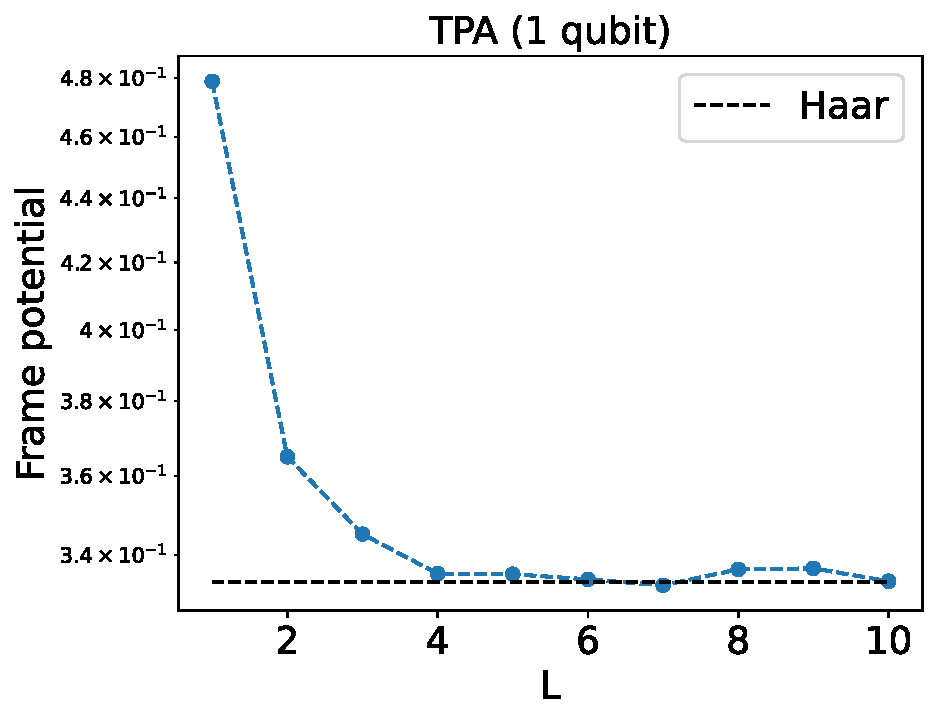
\includegraphics[width=9cm]{1qubit-tpa-exp.pdf}
    \caption{1量子ビットの Tensor Product Ansatz のフレームポテンシャル。黒の破線は量子回路がユニタリ $2$--デザインを成す場合のフレームポテンシャル($=1/3$)である。}
    \label{fig:1qubit-tpa-exp}
\end{figure}


\begin{figure}[H]
    \begin{minipage}[b]{0.5\columnwidth}
        \centering
        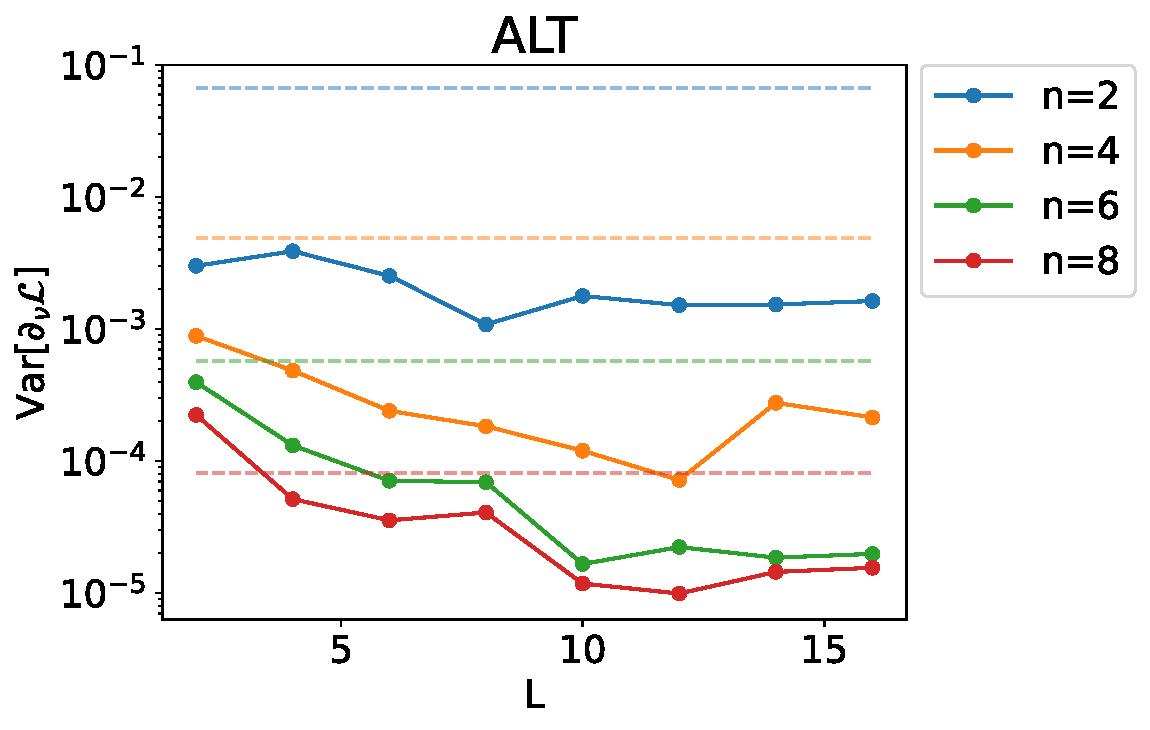
\includegraphics[width=8.5cm]{qml-var-alt.pdf}
    \end{minipage}
    \hspace{0\columnwidth}
    \begin{minipage}[b]{0.5\columnwidth}
        \centering
        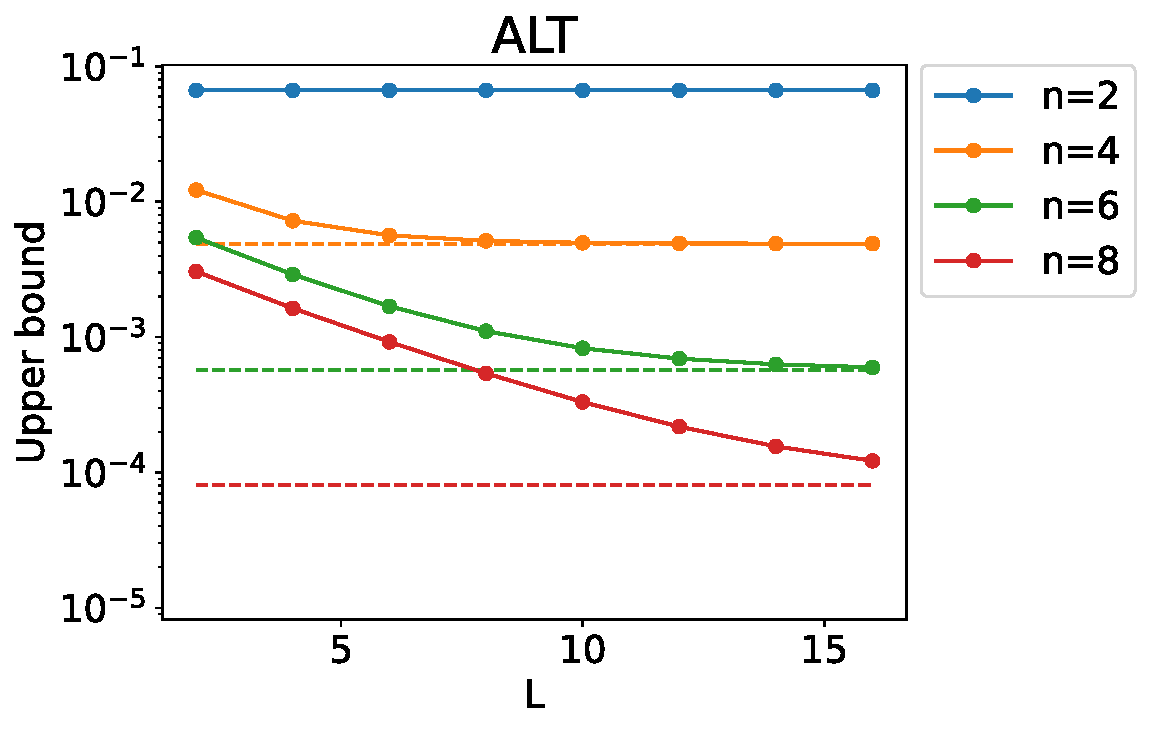
\includegraphics[width=8.5cm]{qml-var-bound-alt.pdf}
    \end{minipage}
    \caption{入力回路に ALT を用いた場合のコスト関数の勾配の分散(左)とその上界(右)}
    \label{fig:qml-var-alt}
\end{figure}

我々は、特にデータの入力が勾配の分散に与える影響に興味があった。
そこで、上界の表式のうちデータ入力に依存する項 $\int_{U\in\bbU} dU D_{\HS} (\rho^{(h)} , \bbid/2^s)$ だけに着目してプロットすると、図~\ref{fig:hsd-alt-analytical}のようになる。  

解析的には示せていないが、図から曲線はある直線 $\beta^{-L}\,(1 < \ex\beta)$ を下回らないことが分かる。よって、上界が量子ビット数 $n$ に対して指数関数的に落ちないためには、ある $\gamma$ に対して $n^{-\gamma} < \beta^{-L}$、すなわち、$L < \gamma\log{n}/\log\beta$ である必要がある。これが、入力回路に Alternating Layered Ansatz を用いた場合に、バレンプラトーが起きないための必要条件である。
以上から、バレンプラトーが起きないためには学習回路が浅いことに加えて、入力回路も $\order{\log{n}}$ 程度に浅くなければならないことが分かる。

\begin{figure}[H]
    \centering
    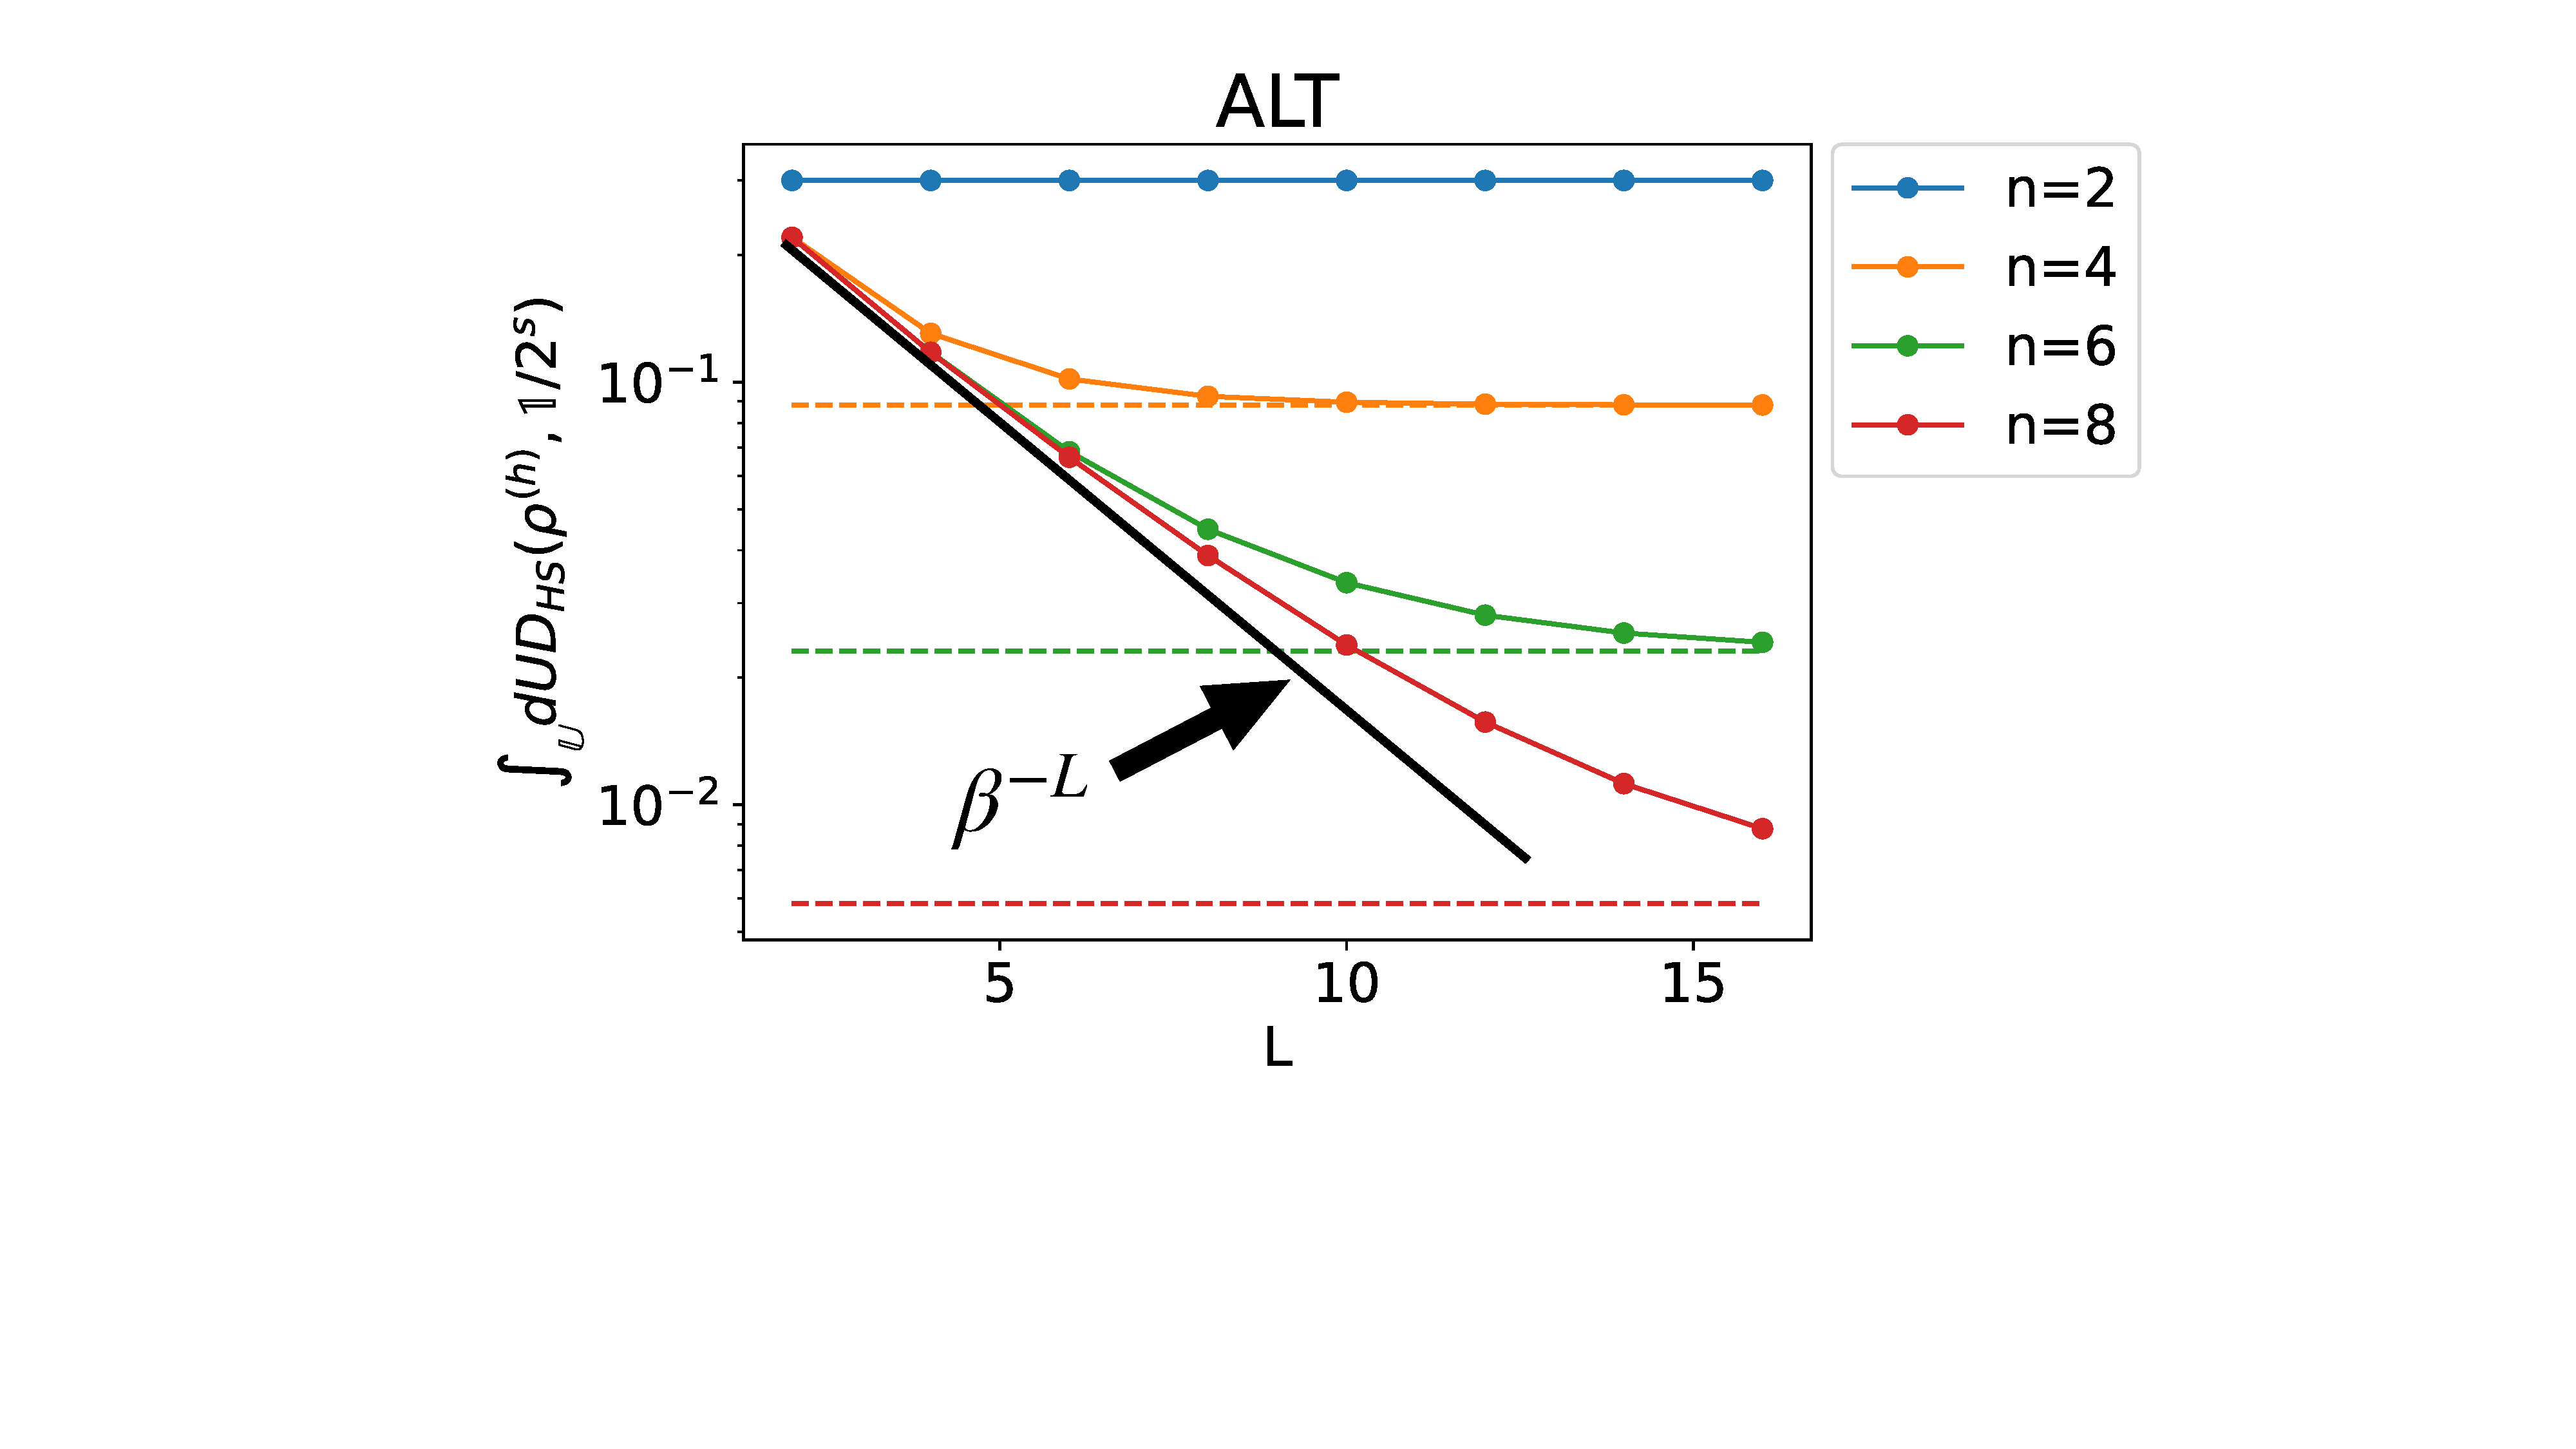
\includegraphics[width=11cm]{hsd-alt-analytical-with-line.pdf}
    \caption{入力回路に ALT を用いた時の $\int_{U\in\bbU} dU D_{\HS} (\rho^{(h)} , \bbid/2^s)$ の計算結果}
    \label{fig:hsd-alt-analytical}
\end{figure}


\section{ノイズの影響}\label{sec:qml-var-noise}
ここまでのコスト関数の勾配の分散の計算においては、ノイズは考慮していなかった。しかし、実際の量子コンピューターにはノイズが存在し、ノイズはバレンプラトーの原因の1つでもある。そこで、ノイズの影響も考慮した場合に、コスト関数の勾配の分散の上界がどのように変化するかを調べる。具体的には、\ref{sec:qml-var-local-2-design}~節で行った計算に Depolarizing ノイズを仮定して、コスト関数の勾配の分散の上界を計算する。
各層のユニタリチャネル $\calE_i(\rho) = U_i\rho U_i\dg,\, i = 1,\,2,\,\cdots,\,L$ に付随して、次の Depolarizing noise channel $\calN_p$ を作用させることを考える。
\begin{align*}
    \calN_p(\rho) = (1-p)\rho + \frac{p}{d}\,\bbid
\end{align*}

このとき、全体のチャネル $\calN = \bigcirc_{i=1}^L \calN_{p} \circ \calE_i$ は次のように表されることを既に確認した(\ref{sec:depolarizing-channel}~節)。
\begin{align*}
    \calN(\rho)
    = (1 - p)^L\calE(\rho) + \{1 - (1 - p)^L\}\,\frac{\bbid}{2^n}
\end{align*}
ただし、$\calE := \bigcirc_{i=1}^L \calE_i$ である。

$D_{HS}(\rho,\,\bbid/d) = \Tr[\rho^2] - \frac{1}{d}$ であることを用いると、
\begin{align}
    D_{HS}(\calN(\rho),\,\bbid/d)
    &= \Tr[\calN(\rho)^2] - \frac{1}{d}\nonumber\\
    &= (1-p)^L\qty{(1-p)^L\Tr[\rho^2] - \frac{1}{d}}\nonumber\\
    &\leq (1-p)^L\qty{\Tr[\rho^2] - \frac{1}{d}}\nonumber\\
    &= (1-p)^L\,D_{HS}(\rho,\,\bbid/d).
\end{align}

したがって、ノイズの影響を考慮した場合のコスト関数の勾配の分散の上界は、次のようになる。
\begin{align}
    \Var_{V(\bs{\th})}[\pd_\nu \calL_{\text{noise}}(\bs{\th})]
    &\leq
    2\max_{i,\bs{\th}} [(\pd_{\ell_i(\bs{\th})}f)^2]
    \times r_{n,s} \times
    \int_{U\in\bbU} dU D_{\HS} (\calN(\rho^{(h)}) , \bbid/2^s)\nonumber\\
    &\leq
    2\max_{i,\bs{\th}} [(\pd_{\ell_i(\bs{\th})}f)^2]
    \times r_{n,s} \times
    (1-p)^L\int_{U\in\bbU} dU D_{\HS} (\rho^{(h)} , \bbid/2^s)\label{eq:qml-var-bound-noise}
\end{align}

図~\ref{fig:qml-var-alt}の右はノイズがある場合の上界\eqref{eq:qml-var-bound-noise}をプロットしたものである。
また、\ref{sec:qml-var-local-2-design}~節と同じ設定の下、Depolarizing ノイズ ($p=0.03$)を加えてアヤメの分類問題のコスト関数の勾配の分散を計算すると、図~\ref{fig:qml-var-alt-noise}の左のようになった。
勾配の分散の計算のために、全てのパラメーターを $10$ 回ランダムにサンプリングした。ただし、プロットしたのは、学習回路の各パラメーターに関する勾配の分散 $\Var[\pd_{\th_i} \calL(\bs{\th})]$ を $i$ について平均したものである。
図~\ref{fig:qml-var-alt}と比較すると、コスト関数の勾配の分散がさらに小さくなっていることが分かる。
上界のノイズに依る項 $(1-p)^L$ だけを見ても、バレンプラトーが起きないためには $L \in \order{\log{n}}$ でなければならないことが分かる。
\begin{figure}[H]
    \begin{minipage}[b]{0.5\columnwidth}
        \centering
        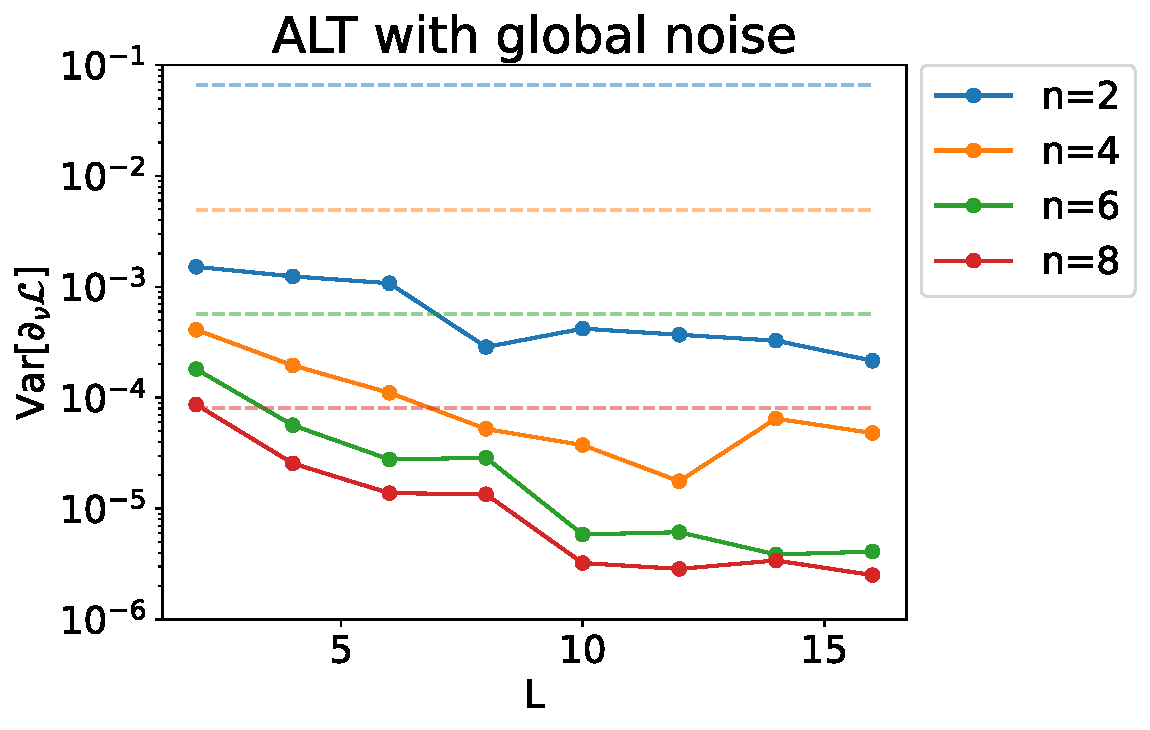
\includegraphics[width=8.5cm]{alt-var_global-noise.pdf}
        % \caption{ALT:ノイズなしのコスト関数の勾配の分散}
    \end{minipage}
    \hspace{0\columnwidth}
    \begin{minipage}[b]{0.5\columnwidth}
        \centering
        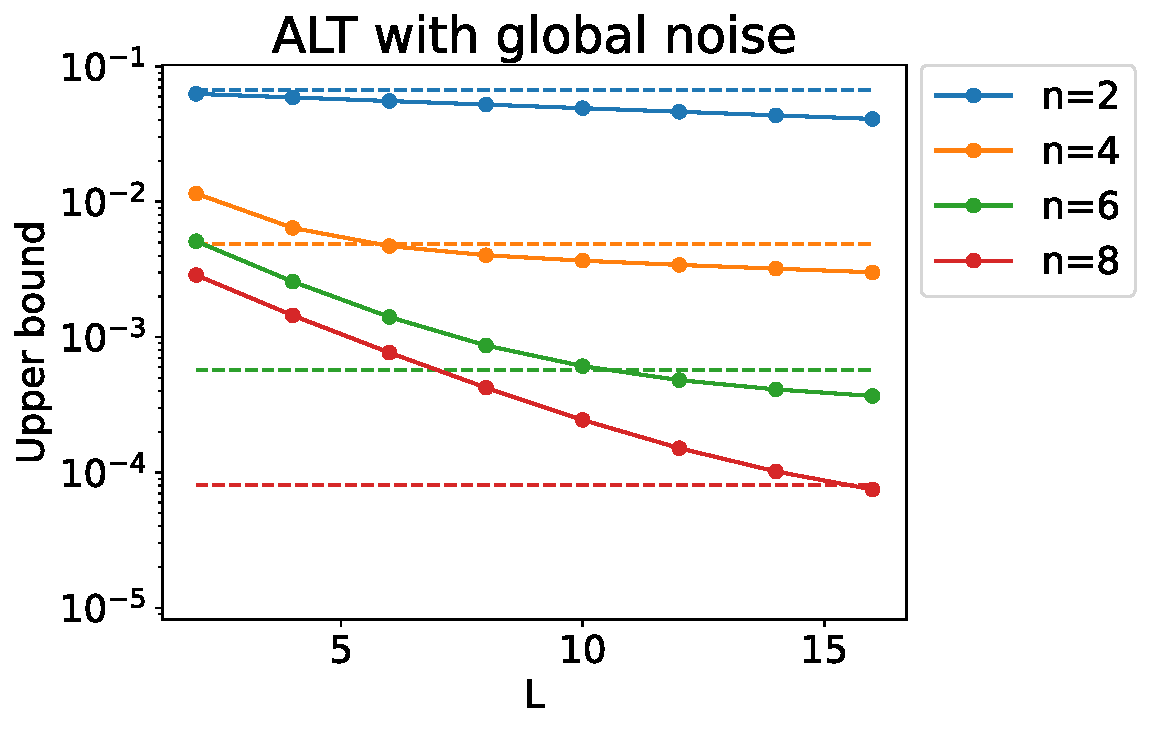
\includegraphics[width=8.5cm]{alt-var-bound_global-noise.pdf}
    \end{minipage}
    \caption{ノイズのある入力回路に ALT を用いた場合のコスト関数の勾配の分散(左)とその上界(右)}
    \label{fig:qml-var-alt-noise}
\end{figure}
